\documentclass[]{article}
\RequirePackage{amsmath}

\usepackage{graphicx}
\usepackage{amssymb}
\usepackage{color}
\usepackage{hyperref}
\usepackage{float}
\usepackage{algorithm}
\usepackage{algpseudocode}

\bibliographystyle{IEEEtran}

\newcommand{\knote}[1]{{\textcolor{green}{Alex notes:{#1}}}}
\newcommand{\dnote}[1]{{\textcolor{red}{DNotes:{#1}}}}
\newcommand{\Ergo}{Ergo}
\newcommand{\Erg}{\textbf{Erg}}
\newcommand{\nanoErg}{\textbf{nanoErg}}
\def\Let#1#2{\State #1 $:=$ #2}
\def\LetRnd#1#2{\State #1 $\gets$ #2}

\begin{document}
    \title{Ergo: A Resilient Platform For Contractual Money}
    \author{Ergo Developers}

    %    \date{January 25, 2019\\v1.0}

    \maketitle

    \begin{abstract}
        We present Ergo, a new flexible blockchain protocol.
        Ergo is designed for developing decentralized applications with the main focus of providing an efficient, secure and easy way to implement financial contracts.

        To achieve this goal, Ergo includes various technical and economic improvements to existing
        blockchain solutions. Every coin in Ergo is protected by a program in ErgoScript, which is
        a powerful and protocol-friendly scripting language based on $\Sigma$-protocols.
        Using ErgoScript, we can encode the conditions under which coins may be used: who can spend them,
        when, under what external conditions, to whom, and so on.

        Extended support for light nodes makes Ergo friendly for end users because it allows running 
        contracts on untrusted commodity hardware.
        To be usable in the long-term, Ergo follows a survivability approach -- it uses
        widely-researched solutions that don't result in security issues in the future,
        while also preventing performance degradation over time with the new economic model.
        Finally, Ergo has a self-amendable protocol that allows it to absorb new ideas and
        improve itself in the future.
\end{abstract}

    \section{Introduction}
\label{sec:intro}

% say the WHY creating Ergo. And also attack the existing financial system a few times.
% Important the readers know that Ergo really is in the same spirit of Bitcoin in the sense it is open,
% permissionless and is designed to disintermediate trusted third parties. But then we need to make clear if
% not too directly that Bitcoin/Ethereum still face a lot of challenges that Ergo is built to address.

Beginning more than ten years ago with Bitcoin~\cite{nakamoto2008bitcoin}, blockchain technology has so far proved
to be a secure way of maintaining a public transaction ledger and disintermediating trusted third parties such as 
traditional financial institutions to some degree.
Even after achieving a market capitalization over \$300bn in 2017~\cite{btcPrice},
no severe attacks were performed on the Bitcoin network despite the high potential yield.
This resilience of cryptocurrencies and the financial empowerment and self-sovereignty they promise to bring is
achieved by a combination of modern cryptographic algorithms and decentralized architecture.

However, this resilience comes at a cost 
%does not come for free 
and has not yet been proven for existing systems in the long-run at economy-wide scale.
To use a blockchain without any trust, its participants should check each other by downloading and
processing all the transactions in the network, utilizing network resources.
Besides network utilization, transaction processing also utilizes computational resources,
especially if the transactional language is sufficiently flexible.
Finally, blockchain participants have to keep a significant amount of data in their local storages and
the storage requirements are growing fast.
Of this, certain data must be maintained in memory.
Thus, transaction processing utilizes various resources of hundreds of thousands of computers all over the world
and consumption of these resources is paid for by regular users in the form of transaction fees~\cite{chepurnoy2018systematic}.
Despite the generous block reward subsidy in some existing systems, their fees can still be very high at times~\cite{bitcoinFees}.
Due to this, even after being around for more than ten years, blockchain technology is still primarily being used in financial applications, where the advantage of high security outweighs the disadvantage of high transaction costs.

Besides the vanilla currency example, the other use of blockchains is to build decentralized applications.
Such applications utilize the ability of the underlying platform to write smart contracts~\cite{szabo1994smart} implementing their logic by means of a blockchain-specific programming language.
One way to classify blockchains in terms of their ability to write smart contracts is based on if they are  
{\em UTXO-based}~(e.g., Bitcoin) or {\em account-based}~(e.g., Ethereum)~\cite{zahnentferner2018chimeric}.
Account-based cryptocurrencies, such as Ethereum, introduce special contract accounts controlled by code,
that may be invoked by incoming transactions.
Although this approach allows performing arbitrary computation, the implementation of complex spending conditions
can lead to bugs such as the one in an Ethereum's ``simple'' multi-signature contract that caused a loss of \$150 million in 2017~\cite{parityLock}.
In UTXO-based cryptocurrencies, every coin has a script associated with it, and to spend that coin, one must satisfy the conditions given in the script.
Implementing such protecting conditions is much easier with the UTXO model but doing arbitrary Turing-complete computation is quite complex~\cite{chepurnoy2018self}.
However, most financial contracts do not require Turing-completeness~\cite{jansenDo}.
Ergo is based on the UTXO model and provides a convenient way to implement financial applications covering an
overwhelming majority of public blockchain use-cases.

While the contractual component is important for building decentralized applications,
it is also essential that the blockchain survives in the long-term.
Application-oriented blockchain platforms have existed only for a few years and the whole area is quite young. Since such platforms have already encountered problems with performance degradation over time~\cite{???}, their long-term survivability is questionable.
Even older UTXO-based money-oriented blockchains have not been proven to be fully resilient in the long-run
under changing conditions because we only have about 10 years of blockchain history up to this point.
Solutions for long-term survivability include concepts 
such as light nodes with minimal storage requirements~\cite{reyzin2017improving},
storage-rent fee component to prevent bloating of full-nodes~\cite{chepurnoy2018systematic}, and 
self-amendable protocols that can adapt to the changing environment and improve themselves without
trusted parties~\cite{goodman2014tezos}.
What is needed is a combination of various scientific ideas together to fix these problems, while also
providing a way for further improvements without any breaking changes and this is exactly what Ergo seeks to accomplish.


    \section{Ergo Vision}
\label{sec:social}

%\knote{Ergo Vision And The Social Contract ?}
%\dnote{May be just Ergo Vision? }

The \Ergo{} protocol is very flexible and may be changed in the future by the community.
In this section we define the main principles that should be followed in Ergo which
might be referred to as ``Ergo's Social Contract''.
In case of intentional violation of any of these principles, the resulting protocol should not
be called \Ergo{}.


\begin{itemize}
    \item{\em Decentralization first.} \Ergo{} should be as decentralized as possible: any parties (social leaders, software developers, hardware manufacturers, miners, funds and so on)
    whose absence or malicious behavior may affect the security of the network should be avoided.
    If any of these parties do appear during \Ergo{}'s lifetime, the community should consider ways to decrease their impact level.
    \item{\em Created for regular people.} \Ergo{} is a platform for ordinary people, and their interests should not be infringed upon in favor of big parties.
    In particular, this means that centralization of mining should be prevented and regular people should be able to participate in the protocol by running a full node and mining blocks (albeit with a small probability).
    \item{\em Platform for Contractual money.} \Ergo{} is the base layer to applications that will be built on top of it.
    It is suitable for several applications but its main focus is to provide an efficient, secure and easy way to implement financial contracts.
    \item{\em Long term focus.} All aspects of \Ergo{} development should be focused on a long term perspective.
    At any point of time, \Ergo{} should be able to survive for centuries without expected hard forks,
    software or hardware improvements or some other unpredictable changes.
    Since Ergo is designed as a platform, applications built on top of Ergo should also be able to survive in the long term.
    This resiliency and long term survivability may also enable Ergo to be a good store of value.
    \item{\em Permissionless and open.} \Ergo{} protocol does not restrict or limit any categories of usage.
    It should allow anyone to join the network and participate in the protocol without any preliminary actions.
    Unlike the traditional financial system, no bailouts, blacklists or other forms of discrimination should be possible
    on the core level of \Ergo{} protocol.
    On the other hand application developers are free to implement any logic they want, taking responsibility for the ethics and legality of their application.
\end{itemize}

    \section{Autolykos Consensus Protocol}
\label{sec:autolykos}

The core component of any blockchain system is its consensus protocol and Ergo utilizes a self-developed
unique Proof of Work (PoW) consensus protocol called {\em Autolykos}, which is described below.
Despite extensive research on possible alternatives, the original PoW protocol with the longest chain rule is still in demand due to its simplicity, high-security guarantees, and friendliness to light clients.
However, a decade of extensive testing has revealed several problems with the original one-CPU-one-vote idea.

The first known problem of a PoW system is the development of specialized hardware (ASICs), which allows a small group of ASIC-equipped miners to solve PoW puzzles orders of magnitude faster and more efficiently than everyone else. This problem can be solved with the help of memory-hard PoW schemes that reduce the disparity between ASICs and commodity hardware. The most promising approach here is to use asymmetric memory-hard PoW schemes that require significantly less memory to verify a solution than to find it~\cite{biryukov2017equihash,ethHash}.

The second known threat to a PoW network decentralization is that even big miners tend to unite in
mining pools, leading to a situation when just a few pool operators (5 in Bitcoin, 2 in Ethereum
at the time of writing) control more than 51\% of computational power.
Although the problem has already been discussed in the community, no practical solutions have been
implemented before \Ergo{}.


Ergo's PoW protocol, Autolykos~\cite{Ergopow}, is the first consensus protocol that is both memory-hard
and pool-resistant.
Autolykos is based on the {\em one list $k$-sum problem}: a miner has to find
$k=32$ elements from a pre-defined list $R$ of size $N=2^{26}$~(which has a size of 2 Gb),
such that $\sum_{j \in J} r_{j} - sk = d$ is in the interval $\{-b,\dots,0,\dots,b\mod q\}$.
Elements of list $R$ are obtained as a result of one-way computation from index $i$,
two miner public keys $pk,w$ and hash of block header $m$ as $r_i=H(i||M||pk||m||w)$,
where $H$ is a hash function which returns the values in $\mathbb{Z}/q\mathbb{Z}$ and
$M$ is a static big message that is used to make hash calculation slower.
Also, a set of element indexes $J$ is to be obtained
by one-way pseudo-random function $genIndexes$, that prevents possible solutions
search optimizations.

Thus, we assume that the only option for a miner is to use the simple brute-force method given in Algorithm~\ref{alg:prove} to
create a valid block.

\begin{algorithm}[H]
    \caption{Block mining}
    \label{alg:prove}
    \begin{algorithmic}[1]
        \State \textbf{Input}: upcoming block header hash $m$, key pair $pk=g^{sk}$
        \State Generate randomly a new key pair $w=g^x$
        \State Calculate $r_{i \in [0,N)}=H(i||M||pk||m||w)$
        \While{$true$}
        \LetRnd{$nonce$}{$\mathsf{rand}$}
        \Let{$J$}{$genIndexes(m||nonce)$}
        \Let{$d$}{$\sum_{j \in J}{r_j} \cdot x - sk \mod q$}
        \If{$d < b$}
        \State \Return $(m,pk,w,nonce,d)$
        \EndIf
        \EndWhile
    \end{algorithmic}
\end{algorithm}

Note that although the mining process utilizes private keys, the solution itself
only contains public keys. Solution verification is done by Algorithm~\ref{alg:verify}.

\begin{algorithm}[H]
    \caption{Solution verification}
    \label{alg:verify}
    \begin{algorithmic}[1]
        \State \textbf{Input}: $m,pk,w,nonce,d$
        \State require $d < b$
        \State require $pk,w\in \mathbb{G}$ and $pk,w \ne e$
        \Let{$J$}{$genIndexes(m||nonce)$}
        \Let{$f$}{$\sum_{j \in J} H(j||M||pk||m||w)$}
        \State require $w^f = g^d \cdot pk$
    \end{algorithmic}
\end{algorithm}

This approach prevents mining pool formation because the secret key $sk$ is needed for mining: once any pool miner finds a correct solution, he can use this secret to steal the block reward. On the other hand, it is secure to reveal a single solution, as it only contains public keys and reveals a single linear relation between the 2 secrets $sk, w$.

Memory-hardness follows from the fact that Algorithm~\ref{alg:prove} requires keeping
the whole list $R$ for the main loop execution.
Every list element takes 32 bytes, so the whole list of $N$ elements
takes $N \cdot 32 = 2 Gb$ of memory for $N = 2^{26}$.
A miner can try to reduce memory requirements by calculating these elements ``on the fly''
without keeping them in memory, however, he'll need to calculate the same
hash $H$ multiple times~(about $10^4$ times for modern GPUs), thereby reducing efficiency and profit.

Calculating the list $R$ is also quite a heavy computational task: our initial implementation~\cite{ergoMiner}
consumes ~25 seconds on Nvidia GTX 1070 to fill all the $2^{26}$ elements of the list.
This part, however, may be optimized if a miner also stores a list of unfinalized hashes $u_{i \in [0,N)}=H(i||M||pk)$
in memory, consuming 5 more Gigabytes of it. In such a case, work to calculate unfinalized hashes should
be done only once during mining initialization while finalizing them and filling the list $R$
for the new header only consumes a few milliseconds~(about 50 ms on Nvidia GTX 1070).

The target parameter $b$ is built-in into the puzzle itself
and is adjusted to the current network hash rate via a difficulty adjustment
algorithm~\cite{meshkov2017short} to keep time interval between block close to 2 minutes.
This algorithm tries to predict the hash rate of an upcoming 1024 blocks long epoch
based on data from the previous 8 epochs via the well-known {\em linear least squares method}. This makes the predictions better than that of the usual difficulty adjustment algorithm and also makes ``coin-hopping'' attacks less profitable.


    \section{Survivability}
\label{sec:survivability}

% well-tested solutions
% voting
% soft-forkability
% storage rent
% light clients (Пробелмы пользователей без легких клиентов, Дайджест узлы, nipopow/flight clients)

Being a platform for contractual money, Ergo should also support long-term contracts for a
period of a person's life.
At the same time, even young existing smart contract platforms are experiencing issues with performance degradation and
adaptability to external conditions.
This leads to a situation when a cryptocurrency depends on a small group of developers
that should provide a fixing hard-fork, or the cryptocurrency won't survive.

The first common survivability issue is that in pursuit of popularity blockchain developers implement ad-hoc
solutions without proper preliminary research and testing.
Such solutions inevitably lead to bugs, hasty bug fixes, fixes of bug fixes and so on, making the network even less secure.
Ergo approach here is to use stable well-tested solutions, even if that leads to slower
short-term innovation applicability.
Most of Ergo solutions are formalized in scientific papers, presented at peer-reviewed conferences
and are widely discussed in the community.

Ergo is trying to fix known problems of blockchain technology without creating new problems.
As far as Ergo is a PoW blockchain, it easily allows extracting a small header from the block content.
Single header allows validating the work done, while headers chain is enough to select the best chain
and synchronize the network.
Headers chain is much smaller than the full one, however it still growths linearly with time.
Hopefully, modern research of light clients~\cite{kiayias2017non,luuflyclient} provide a way to
synchronize the network by downloading an even smaller piece of data, unlocking the ability to
use the network without any trust from low-end hardware like mobile phones.
Also, Ergo uses authenticated state\cite{reyzin2017improving} and for any transaction included
a client may download a proof of its correctness.
This proof is generated by the block miner and allows to check all the state transitions:
transaction inputs were present in the state before its application,
transaction outputs were added after its application and no more changes were done to the state.
Thus, regardless of the blockchain size a regular user with
a mobile phone can join the network and start using Ergo with the same security
guarantees as a full node.

Although support of light clients solves problems of Ergo users, it does not solve problems
of Ergo miners that still should keep the whole state for efficient
transaction validation.
In existing blockchain systems, users can put arbitrary data to this state forever,
creating a lot of dust in it and increasing its size over time~\cite{perez2019another}.
Big state size leads to serious security issues, as far as when the state does not fit in memory,
an adversary may generate transactions which validation become very slow due to required random
access to miners storage
leading to DoS attack like an attack to the Ethereum network in 2016~\cite{??}.
To prevent this Ergo have a storage rent component: if an
output remains in the state for 4 years without being moved a miner may charge a small fee for every
byte kept in the state.
This idea is similar to regular cloud storage services however, it was only proposed quite recently for
cryptocurrencies~\cite{chepurnoy2017space} and has several important consequences.
First, Ergo mining will always be stable unlike Bitcoin and other PoW currencies
in which mining may become unstable after the
initial emission~\cite{carlsten2016instability}.
Second, state size growth becomes controllable and predictable reducing hardware requirements for Ergo miners.
Third, by collecting a storage fee from outdated boxes, miners return coins to circulation preventing a steady decrease
of circulating supply due to lost keys~\cite{wsj2018}.
All these effects should support Ergo long-term survivability, both technically and economically.

Another vital aspect of survivability is that the environment changes and a network should
adapt to changing hardware infrastructure, appearing ideas that may improve security or
scalability, arising use-cases and so on.
If all the rules are fixed without any ability to change them in a decentralized manner, even
simple constant change may lead to huge debates and community split, e.g., discussion of a block
size limit in Bitcoin led to the network split into several independent coins.
In contrast, Ergo protocol is self-amendable and is able to adapt to the changing environment.
In Ergo parameters like block size can be changed on-the-fly via miners voting.
At the beginning of a 1024 blocks length voting epoch miner is proposing changes~(up to 2 parameters,
e.g., to increase block size and to decrease storage fee factor) and during the rest of the epoch miners
vote whether to approve these changes or not.
If the majority of votes within an epoch are supporting some~(or both) of these changes, a new value of
the parameter should be written into the extension section of the first block of the next epoch and
the network starts to use this update parameter value during block mining and validation.

To absorb more fundamental changes, Ergo is following the approach of soft-forkability, that
allows to change protocol significantly but keeping old nodes operating.
At the beginning of an epoch, a miner can also propose to vote for a fundamental change~(e.g., to add a new instruction to ErgoScript), describing affected validation rules.
Voting for such breaking changes continues for 32768 blocks and requires at least $90\%$ of
"Yes" votes to be accepted.
Once being accepted, 32768 blocks length activation period started to give time to outdated
nodes to update their software version.
If a node is still not updated after the activation period, it skips the specified checks,
however, continues to validate all the known rules.
List of previous soft-fork changes is recorded into the extension to allow light nodes of
any software version to join the network and read current validation rules.

    \section{Ergo's Native Token}

 \dnote{Bitcoin have utility usage to pay for network resources as well as Ethereum has a utility usage to pay for
 computations~(we've also discussed it in "Systematic approach to cryptocurrency fees" paper). Also Ethereum emission
 rate was only reduced making it better and better as a store of value and is following "set in stone social contract" that
 it will reach zero when it will switch to PoS. Keeping in mind lost coins, Ethereum may be better then Ergo even
 right now, as far as efficient number of coins in circullation may reduce with time unlike Ergo.}

 \dnote{Instead of comparision of medium of exchange or store of value properties with BTC/ETH, I propose to
 describe, that Erg is utility token with the different purpose~(pay storage fee) and also have limited
 supply~(that would be natural if we'll move this part into previous section)}

 \knote{I disagree, but you are free to propose an alternative text. Also, what was discussed in the "Systematic
 approach..." paper that is a fee structure, not usefulness of a token.}

 In this section, we provide some reflections on the nature of the native Ergo token. For starters, we note that
 any currency has three main functions: a medium of exchange, a unit of account, and a store of value.

 Bitcoin, being historically the first digitally scarce asset, is perfect as store-of-value. It is even better than gold under certain assumptions~(such as the SHA-256 hash function not being broken, and a majority of miners not willing to destroy Bitcoin), as emission is limited and known in advance. However, being the perfect store-of-value also means that it is not so good as medium-of-exchange. In particular, if one knows that Bitcoin is indeed the best tool to store value in the long term, he would use fiat whenever possible to collect more bitcoins.

 On the other hand, Ethereum is not just a currency, but a utility token used to pay for computations over the
``decentralized world computer'' (or ``fully replicated programmable calculator''). However, Ethereum is not good as
 store-of-value, as emission is endless, and, historically, can be changed easily by the community along with critical system parameters.

 Ergo combines best from these two top blockchains. Emission is predefined and limited. Furthermore, it will be finished within
 just ten years. The system assumptions are set in stone with a precisely defined {\em social contract}~\ref{sec:social}. Also,
 Ergo is a utility token used to pay storage rent. This storage rent makes the system more stable. Lastly, Ergo is suitable for building monetary systems on top of it with properties different from the Ergo native token itself. However, participating in such systems would require using the Ergo native token as well in order to pay storage rent.


\subsection{Currency And Emission}
\label{sec:currency}

The native currency of \Ergo{} platform is the \Erg{} token, whose unique property is
that it is the only currency for paying storage rent in \Ergo{}~(see Section~\ref{sec:survivability} for more details).
One \Erg{} is divisible to up to $10^9$ smaller units, called \nanoErg{}s.

All \Erg{} tokens that will ever circulate in the system are present in
the initial state and are divided into 3 parts~(boxes):

\knote{no any notion of a box was introduced before, the introduction is sudden}
\dnote{I propose to add section about Ergo state before this one and introduce box notion in it}

\begin{itemize}
    \item{\em No premine proof.} This box contains exactly one~\Erg{} and is protected by a script that prevents it from being spent by anyone.
    Thus, it is a long-lived box that will stay in the system until the storage-rent component
    destroys it.
    Its main purpose is to prove that \Ergo{} mining was not started privately by anyone before
    the declared launch date.
    To achieve this, additional registers of this box contain latest headlines from the media (The Guardian, Vedomosti, Xinhua), as well as the latest block identifiers from Bitcoin and Ethereum.
    Thus, \Ergo{} mining could not have started before certain events in the real world and the cryptocurrency space.

    \item{\em Treasury.} This box contains 4,330,791.5 \Erg{} that will be used to fund \Ergo{}
    development.
    Its protecting script~\cite{link to corresponding ergo tree} consists of two parts.

    First, it ensures that only a predefined portion of the box value is unlocked.
    During blocks 1-525,599 (2 years) 7.5 \Erg{} will be released every block. Then during blocks 525,600-590,399 (3 months) 4.5 \Erg{} will be released every block. Finally, 
    during blocks 590,400-655,199 (3 months) 1.5 \Erg{} will be released every block.
    This rule ensures the presence of funds for \Ergo{} development for at least 2.5 years and, at any moment of time,
    rewards do not exceed 10\% of the total number of coins in circulation.

    Second, it has custom protection from unexpected spending.
    Initially, it requires the spending transaction to be signed by at least 2 of 3 secret keys that are under control of the initial team members. When they spend the box, they are free to
    change this part of the script as they wish, for example by adding new members to protect foundation
    funds.

    During the first year, these funds will be used to cover the pre-issued EFYT token~\cite{our website with swap }. After that they will be distributed in a decentralized manner via a community voting system that is under development.


    \item{\em Miners reward.} This box contains 93,409,132 \Erg{} that will be collected by block miners
    as reward for their work.
    Its protecting script~\cite{link to corresponding ergo tree} requires the spending transaction to have exactly two outputs with the following properties:

    \begin{itemize}
    \item{} The first output should be protected by the same script and the number of \Erg{} in it should
    equal to the remaining miners' reward.
    During blocks 1 - 525,599 (2 years), a miner will be able to collect 67.5 \Erg{} from this box. During blocks 525,600 - 590,399 (3 month), a miner will be able to collect 66 \Erg{}, and after that, the block reward will be reduced by 3 \Erg{} every 64,800 blocks (3 months) until it reaches zero at block 2,080,799.

    \item{} The second output should contain the remaining coins and should be protected by the following condition:
    it can be spent by a miner that solved the block's PoW puzzle and not earlier than 720 blocks after the current block.
    % These restrictions are done to prevent mining pools formation, see~\ref{sec:autolykos} for more details.
    \end{itemize}

\end{itemize}

All these rules results in the following curve denoting the number of coins in circulation with time:

\begin{figure}[H]
    \centering
    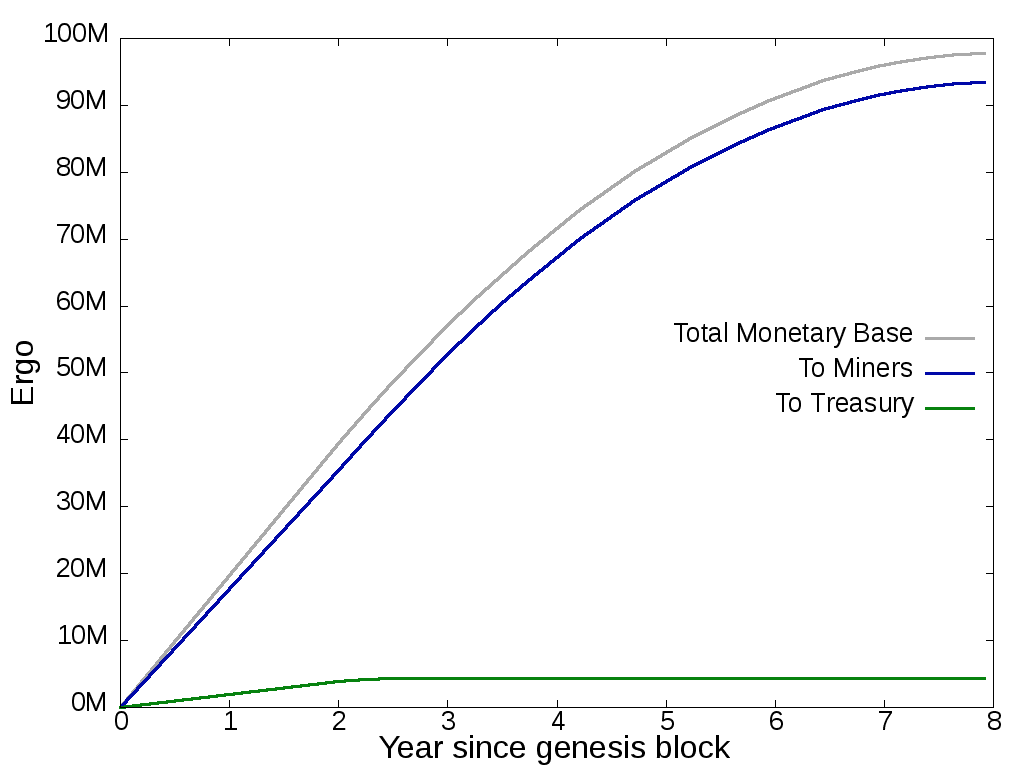
\includegraphics[width=\textwidth]{img/emission.png}
    \caption{Ergo emission curve
    \label{fig:emission} }
\end{figure}


    

\section{Contractual Money}
    \label{sec:contractual}

 In our opinion, the overwhelming majority of use-cases for a public blockchains (even those that claim to provide a general-purpose decentralized world computer) are for financial applications, which do not require Turing-completeness. For instance, if an oracle writes down non-financial data into the blockchain~(such as temperature), this data is usually used further in a financial
 contract. Another trivial observation we make is that many applications use digital tokens with mechanics different from the native token.

For an application developer, the Ergo Platform offers custom tokens~(which are first-class citizens) and a domain-specific language for writing box protecting
 conditions in order to implement flexible and secure financial applications.
 Ergo applications are defined in terms of protecting scripts built into boxes, which may also contain data involved in the execution.
 We use the term {\em contractual money} to define Ergs (and secondary tokens) whose usage is bounded by a contract. This applies to all tokens on the platform in existance because any box with its contents~(Ergs, tokens, data) is bounded by a contract.
 
 However, we can distinguish between two types of contractual Ergs. The first, called {\em free Ergs}, are the ones that could change their contracts easily and have no restrictions on the outputs or the other inputs of a spending transaction. The second type are {\em bounded Ergs}, whose contracts require the spending transaction to have input and output boxes with specific properties. 
 
 For example, if a box $A$ is protected by just a public key~(so providing a signature against a spending transaction is enough in order to destroy the box), the public key owner can spend $A$ and transfer the Ergs to any arbitrary output box. Thus, the Ergs within $A$ are free. 
% to change the contract. 
In contrast, imagine a box $B$ protected by combination of a public key and a condition that demands the spending transaction to create an output box with the same amount of Ergs as in $B$ and whose guarding script has the hash \texttt{rBMUEMuPQUx3GzgFZSsHmLMBouLabNZ4HcERm4N} (in Base58 encoding). In this case, the Ergs in $B$ are bounded Ergs.
 
 Similarly, we can define free and bounded tokens. An Ergo contract can have several hybrids such as bounded Ergs and free tokens or both bounded under one public key and free under another.

\subsection{Preliminaries For Ergo Contracts}

  While in Bitcoin, a transaction output is protected by a program in a stack-based language named {\em Script}, in Ergo a box is protected by a logic formula which combines predicates over a context with cryptographic statements provable via zero-knowledge protocols using AND, OR, and $k$-out-of-$n$ connectives. The formula is represented as a typed direct
 acyclic graph, whose serialized form is written in a box. To destroy a box, a spending transaction needs to provide arguments (which include zero-knowledge proofs) satisfying the formula.

 However, in most cases, a developer is unlikely to develop contracts in terms of graphs. Instead, he would like to use a high-level language such as ErgoScript, which we provide with the reference client. 
 
 Writing scripts in ErgoScript is easy. As an
 example, for a one-out-of-two signature, the protecting script would be ${pk_1 \|pk_2}$, which means ``prove knowledge of
 a secret key corresponding to the public key $pk_1$ or knowledge of a secret key corresponding to public key $pk_2$''. We have
 two separate documents for help in developing contracts with ErgoScript: the ``ErgoScript Tutorial''~\cite{ergoTutorial}
 and the ``Advanced ErgoScript Tutorial''~\cite{ergoAdvTutorial}. Thus, we do not get into the details of developing contracts with ErgoScript. Rather, we provide a couple of motivating examples in the following sections.

Two more features of Ergo shaping contracting possibilities are:

 \begin{itemize}
    \item {\em Data Inputs: }
 To be used in a transaction, a box need not be destroyed but can instead be read-only. In the latter case, we refer to the box as being part of the {\em data input} of the transaction. Thus, a transaction gets two box sets as its arguments, the inputs and
 data inputs, and produces one box set named {\em outputs}. Data inputs are useful for oracle applications and interacting contracts.

    \item {\em Custom Tokens: }
 A transaction can carry many tokens as long as the estimated complexity for processing them does not exceed a limit, a parameter that is set by miner voting. A transaction can also issue a single token with a unique identifier which is equal to identifier of a first~(spendable) input box of the transaction. The identifier is unique assuming the collision resistance of an underlying hash function.
 The amount of the tokens issued could be any number within the range $[1, 9223372036854775807]$. The weak preservation rule is followed for tokens, which requires that the total amount of any token in a transaction's outputs should be no more
 than total amount of that token in the transaction's inputs~(i.e., some amount of token could be burnt). In contrast, the strong reservation rule is followed for Ergs, which requires that the total amount of Ergs in the inputs and outputs must be same.
 \end{itemize}

\subsection{Contract Examples}
\label{sec:examples}

 In this section we provide some examples which demonstrate the superiority of Ergo contracts compared to Bitcoin's. The examples include betting on oracle-provided data, non-interactive mixing, atomic swaps, complementary currency, and an initial coin offering implemented on top of the Ergo blockchain.

 \subsubsection{An Oracle Example}
 \label{sec:platform}

 Equipped with custom tokens and data inputs, we can develop a simple oracle example which also shows some design patterns that we discovered while playing with Ergo contracts. Assume that Alice and Bob want to bet on tomorrow's weather by putting money into a box that becomes spendable by Alice if tomorrow's temperature is more than 15 degrees, and spendable by Bob otherwise. To deliver the temperature into the blockchain, a trusted oracle is needed.

 In contract to Ethereum with its long-lived accounts, where a trusted oracle's identifier is usually known in advance, delivering data with one-time boxes is more tricky. For starters, a box protected by the oracle's key cannot be trusted, as anyone can create such a box. It is possible to include signed data into a box and check the oracle's signature in the contract (we have such an example), but this is quite involved. Instead, a solution with custom
 tokens is very simple.

 Firstly, a token identifying the oracle should be issued. In the simplest case, the amount of this token could be one. We call such a token {\em a singleton token}. The oracle creates a box containing this token along with its data (i.e., the temperature) in register $R_4$ and the UNIX epoch time in register $R_5$.
 In order to update the temperature, the oracle destroys its box and creating a new one with the updated temperature.

 Assume that Alice and Bob know the oracle's token identifier in advance. With this knowledge, they can jointly create a box with a contract that requires first (read-only) data input to contain the oracle's token. The contract extracts the temperature and time from the data input
 and decides who gets the payout. The code is as simple as following:

 \begin{algorithm}[H]
    \caption{Oracle Contract Example}
    \label{alg:oracle}
    \begin{algorithmic}[1]
        \State val dataInput = CONTEXT.dataInputs(0)
        \State val inReg = dataInput.R4[Long].get
        \State val inTime = dataInput.R5[Long].get
        \State val inToken = dataInput.tokens(0).\_1 == tokenId
        \State val okContractLogic = (inTime $>$ 1556089223) \&\&
        \State\hspace{\algorithmicindent}\hspace{\algorithmicindent} ((inReg $>$ 15L \&\& pkA) $||$ (inReg $\le$ 15L \&\& pkB))
        \State inToken \&\& okContractLogic
    \end{algorithmic}
 \end{algorithm}

 This contract shows how a singleton token could be used for authentification. As a possible alternative, the oracle
 can put the time and temperature into a box along with a signature on this data. However, this requires signature verification, which is more complex and expensive compared to
 the singleton token approach. Also, the contract shows how read-only data inputs could be useful for contracts which need to access data stored in some other box in the state. Without data inputs, an oracle must issue one spendable box for each
 pair of Alice and Bob. With data inputs, the oracle issues only a single box.

\subsubsection{A Mixing Example}
 \label{sec:platform}

 Privacy is important for a digital currency but implementing it can be costly or require a trusted setup. Thus, it is desirable to find cheaper way for coin mixing. As a first step towards that, we offer a non-interactive mixing protocol between two users Alice and Bob that works as follows:
 \begin{enumerate}
    \item{} Alice creates a box which demands the spending transaction to satisfy certain conditions. After that, Alice only listens to the blockchain, no any interaction with Bob is needed.
    \item{} Bob creates a transaction spending Alice's box along with one of his own and generating two outputs with identical script but different data. Each of Alice and Bob may spend only one of the two outputs but to an external observer the two outputs look indistinguishable and he cannot decide which output belongs to whom.
 \end{enumerate}

 For simplicity, we do not consider fee in the example. The idea of mixing is similar to non-interactive Diffie-Hellman key exchange. First, Alice generates a secret value $x$~(a huge number) and publishes the corresponding public value $gX = g^x$. She requires Bob to generate a secret number $y$, and to include into each output two
 values $c_1$, $c_2$, where one value is equal to $g^y$ and the other is equal to $g^{xy}$. Bob uses a random coin to choose meanings for $\{c_1, c_2\}$. Without access to the secrets, an external observer cannot guess with probability better than  $\frac{1}{2}$ whether $c_1$ is equal to $g^y$ or to $g^{xy}$. This is assuming that the cryptographic primitive we use has a certain property, that the Decision Diffie-Hellman (DDH) problem is hard. To destroy an output box, a proof should be given that either $y$ is known such that $c_2 = g^y$, or $x$ is known such that $c_2 = c_1^x$.
 The contract of Alice's box checks that $c_1$ and $c_2$ are well-formed. The code snippets for the Alice's coin and the mixing transaction's output are provided in Algorithms \ref{alg:alice} and \ref{alg:mixing-out} respectively. Since ErgoScript currently doesn't have support for proving knowledge of some $x$ such that $c_2 = {c_1}^x$ for arbitrary $c_1$,  we will prove a slightly longer statement that is supported, namely, proving knowledge of $x$ such that $gX = g^x$ and $c_2 = {c_1}^x$. This is called proveDHTuple.

 \begin{algorithm}[H]
    \caption{Alice's Input Script}
    \label{alg:alice}
    \begin{algorithmic}[1]
        \State val c1 = OUTPUTS(0).R4[GroupElement].get
        \State val c2 = OUTPUTS(0).R5[GroupElement].get
        \State
        \State OUTPUTS.size == 2 \&\&
        \State OUTPUTS(0).value == SELF.value \&\&
        \State OUTPUTS(1).value == SELF.value \&\&
        \State blake2b256(OUTPUTS(0).propositionBytes) == fullMixScriptHash \&\&
        \State blake2b256(OUTPUTS(1).propositionBytes) == fullMixScriptHash \&\&
        \State OUTPUTS(1).R4[GroupElement].get == c2 \&\&
        \State OUTPUTS(1).R5[GroupElement].get == c1 \&\& \{
        \State\hspace{\algorithmicindent}  proveDHTuple(g, gX, c1, c2) $||$
        \State\hspace{\algorithmicindent}  proveDHTuple(g, gX, c2, c1)
        \State \}
    \end{algorithmic}
 \end{algorithm}

 \begin{algorithm}[H]
    \caption{Mixing Transaction Output Script}
    \label{alg:mixing-out}
    \begin{algorithmic}[1]
        \State val c1 = SELF.R4[GroupElement].get
        \State val c2 = SELF.R5[GroupElement].get
        \State proveDlog(c2) $||$            // either c2 is $g^y$
        \State proveDHTuple(g, c1, gX, c2) // or c2 is $u^y = g^{xy}$
    \end{algorithmic}
 \end{algorithm}

 We refer the reader to \cite{ergoAdvTutorial} for a proof of indistinguishability of the outputs and details on why Alice and Bob can spend only their respective coins.


\subsubsection{More Examples}

 In this section, we briefly shed light on a few more examples along with links to the documents providing the details and code.

\paragraph{Atomic Swap}
Cross-chain atomic swap between Ergo and any blockchain that supports payment to either SHA-256 or Blake2b-256 hash preimages and time-locks can be done in a similar way to that proposed for Bitcoin~\cite{Nol13}. An Ergo alternative implementation is provided in~\cite{ergoTutorial}. As Ergo also has custom tokens, atomic exchange on the single Ergo block chain (Erg-to-token or token-to-token) is also possible. An implementation for this can also be found in~\cite{ergoTutorial}.

\paragraph{Crowdfunding}

 We consider the simplest crowdfunding scenario. In this example, a crowdfunding project with a known public key is considered successful if it can collect unspent outputs with total value not less than a certain amount before a certain height. A project backer creates an output box protected by the following statement: the box can be spent 
 if the spending transaction has the first output box protected by the project's key and amount no less than the target amount.
 Then the project can collect (in a single transaction) the biggest backer output boxes with total value not less than the target amount~(it is possible to collect up to ~22,000 outputs, which is
 enough even for a big crowdfunding campaign). For remaining outputs, it is possible to construct follow-up transactions. The code can be found in~\cite{ergoTutorial}.

\paragraph{The Local Exchange Trading System}

 Here we briefly demonstrate a Local Exchange Trading System (LETS) in Ergo. In such a system, a member of a community may issue community currency via personal debt. For example, if Alice with zero balance is buying something for $5$
 community tokens from Bob, whose balance is zero as well, her balance after the trade would be $-5$ tokens, and
 Bob's balance would be $5$ tokens. Then Bob can buy something using his $5$ tokens, for example, from Carol.
 Usually, in such systems, there is a limit on negative balances (to avoid free-riding).

 Since a digital community is vulnerable to Sybil attacks~(which also enable free-riding), some mechanism is needed to prevent such attacks where Sybil nodes create debts. 
 The simplest solution is to use a committee of trusted managers that approve new members of the community. A trust-less but more complex solution is to use security deposits made in Ergs. For simplicity, we consider the approach with the committee here.
 
 \snote{Give more details/references about Sybil attacks}

 This example contains two interacting contracts. A {\em management contract} maintains a list of community members, and a new member can be added if some a management condition is satisfied  (for example, a threshold
 signature is provided). A new member is associated with a box containing a token that identifies the member. This box, which contains the {\em member contract}, is protected by a special exchange script that requires the spending transaction to do a fair exchange.
 We skip the corresponding code, which can be found in a separate article~\cite{letsTutorial}.
 
 What this contract shows, in contrast to the previous example, is that instead of storing the members list, only a short digest of an authenticated AVL+ tree can be included in the box. This allows reduction in storage requirements for the state. A transaction doing lookup or modification of the member list should provide a proof for AVL+ tree lookup or modification operations. Thus, saving space in the state storage leads to bigger transactions, but this scalability problem is easier to solve.

\paragraph{Initial Coin Offering}

 We discuss an Initial Coin Offering (ICO) example that shows how multi-stage contracts can be created in Ergo. Like most ICOs, our example has three stages. In the first stage, the project raises money in Ergs. In the second stage, the project issues a new token, whose amount equals the number of nanoErgs raised in the first stage. In the third stage, the investors can withdraw issued tokens.

 Note that the first and third stages have many transactions on
 the blockchain, while a single transaction is enough for the second stage. Similar to the previous example, the ICO contract uses an AVL+ tree to store the list of (investor, amount) pairs. The complete code is available at~\cite{icoTutorial}.


\paragraph{More Examples}

 We have even more examples of Ergo applications in \cite{ergoTutorial, ergoAdvTutorial}. These examples include time-controlled emission, cold wallets contracts, rock-paper-scissors game, and many others.

    \section{Conclusions}
    \label{sec:conclusions}

    \bibliography{references}

\end{document}
